
%(BEGIN_QUESTION)
% Copyright 2006, Tony R. Kuphaldt, released under the Creative Commons Attribution License (v 1.0)
% This means you may do almost anything with this work of mine, so long as you give me proper credit

En smart krets brukt for å konvertere utgangen fra en differensiell kapasitanssensor til et DC-spenningssignal er \textit{diode twin-t circuit} vist her:

$$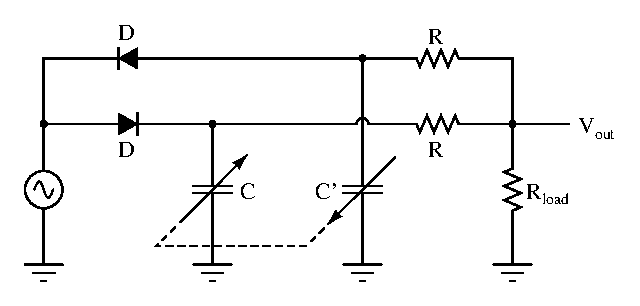
\includegraphics[width=15.5cm]{i00186x01.eps}$$

AC-``eksitasjons''kilden er vanligvis høyfrekvent, minst 1 MHz.  Diodene er hurtigswitchende typer, ideelt Schottky-dioder.  Motstandene $R$ må ha samme verdi, men $R_{load}$ er vanligvis mye større enn $R$.  Sammen danner de to like motstandene ($R$) et \textit{middelverdinettverk} for de to kapasitansene $C$ og $C'$ når de vekselvis utlades gjennom $R_{load}$.

Identifiser hvilken kapasitans ($C$ eller $C'$) som må øke i verdi for å generere en positiv DC-utgangsspenning, og forklar hvorfor.

\underbar{file i00186}
%(END_QUESTION)





%(BEGIN_ANSWER)

Utgangsspenningen vil være positiv i forhold til jord hvis $C > C'$ og negativ hvis $C' > C$.

%(END_ANSWER)





%(BEGIN_NOTES)

Jeg kan ikke ta æren for denne fine lille kretsen.  Jeg fant den på side 72 i {\it Principles of Applied Biomedical Instrumentation} av Geddes og Baker (Copyright 1968, John Wiley and Sons).  Etter å ha brukt den i mitt eget differensialkapasitansmanometer, kan jeg bekrefte at den fungerer veldig godt:

$$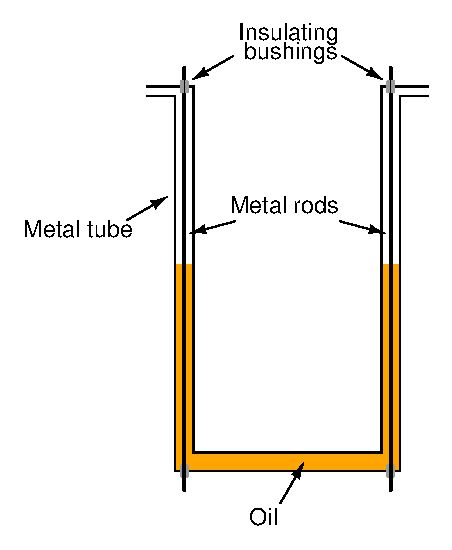
\includegraphics[width=15.5cm]{i00186x02.eps}$$

Dette er et relativt enkelt instrument å bygge med stive kobberrør.  Bruk plast-kompresjonskoblinger som isolerende gjennomføringer.

\vskip 10pt

Det kan være nyttig å repetere denne formelen med studentene når kapasitansbasert instrumentering diskuteres:

$$C = {\epsilon A \over d}$$

\noindent
Hvor,

$C =$ Kapasitans i Farad

$\epsilon =$ Permittivitet i dielektrikum (absolutt)

$A =$ Lederareal, i kvadratmeter

$d =$ Avstand mellom lederne, i meter


%INDEX% Measurement, differential capacitance: twin tee diode circuit

%(END_NOTES)

